\chapter{Opis projektnog zadatka}
\usepackage{graphicx}
\section{Opis projektnog zadatka 'Ples'}

Cilj ovog projekta je razviti programsku podršku za stvaranje web aplikacije “Ples”, koja korisniku olakšava pronalaženje i organizaciju plesnih tečajeva i plesnjaka, time uvelike olakšavajući život ljubiteljima plesa jer će imati sve što im je potrebno u jednoj web aplikaciji

Neregistriranom korisniku se, otvaranjem stranice, prikazuje karta sa dostupnim plesnjacima i lokacijama klubova. Neregistrirani korisnik također može i pregledati profile klubova i tipove plesova koji nudi, a kako bi si olakšao pretragu, plesnjake može filtrirati po tipu plesa, klubu koji ga organizira i tipovima plesa. Isto tako, klubove je moguće filtrirati po tipovima plesa za koje organiziraju tečajeve. 
	Neregistrirani korisnik može kreirati novi račun za klijenta navođenjem sljedećih obaveznih informacija:

\begin{packed_item}
	\item \textit{korisničko ime}
	\item \textit{lozinka}
	\item \textit{ime}
	\item \textit{prezime}
	\item \textit{spol}
	\item \textit{datum rođenja}
	\item \textit{broj mobitela}
	\item \textit{email adresa}
\end{packed_item}

Korisnik također može, ali i ne mora unijeti sljedeće informacije:

\begin{packed_item}
	\item \textit{opis plesnog iskustva}
	\item \textit{fotografija}
\end{packed_item}

\Neregistrirani korisnik također može kreirati novi račun za klub, te će mu za isto biti potrebno navođenje sljedećih informacija:

\begin{packed_item}
	\item \textit{korisničko ime}
	\item \textit{lozinka}
	\item \textit{ime kluba}
	\item \textit{adresa sjedišta}
	\item \textit{broj telefona}
	\item \textit{email}
\end{packed_item}

Nakon stvaranja novog računa za klub, korisnik mora čekati na potvrdu od strane administratora.  Nakon provedene registracije, korisnik može mijenjati sve informacije potrebne za registraciju po volji. Također, korisnik uvijek može izbrisati svoj račun.

Registrirani korisnik može obnašati ulogu klijenta, ulogu kluba, uloge trenera i klijenta ili ulogu administratora.

\underbar{Klijentu} se na karti prikažu i tečajevi slobodni za upis. Rezultate može filtrirati po vremenu i tipu plesa. Sličnu mogućnost nalazimo na web stranici \url{https://danceprogram.duke.edu/courses}, gdje korisnici filtriraju tečajeve po vremenu i vrsti tečaja.

\begin{figure}[H]
	\centering
	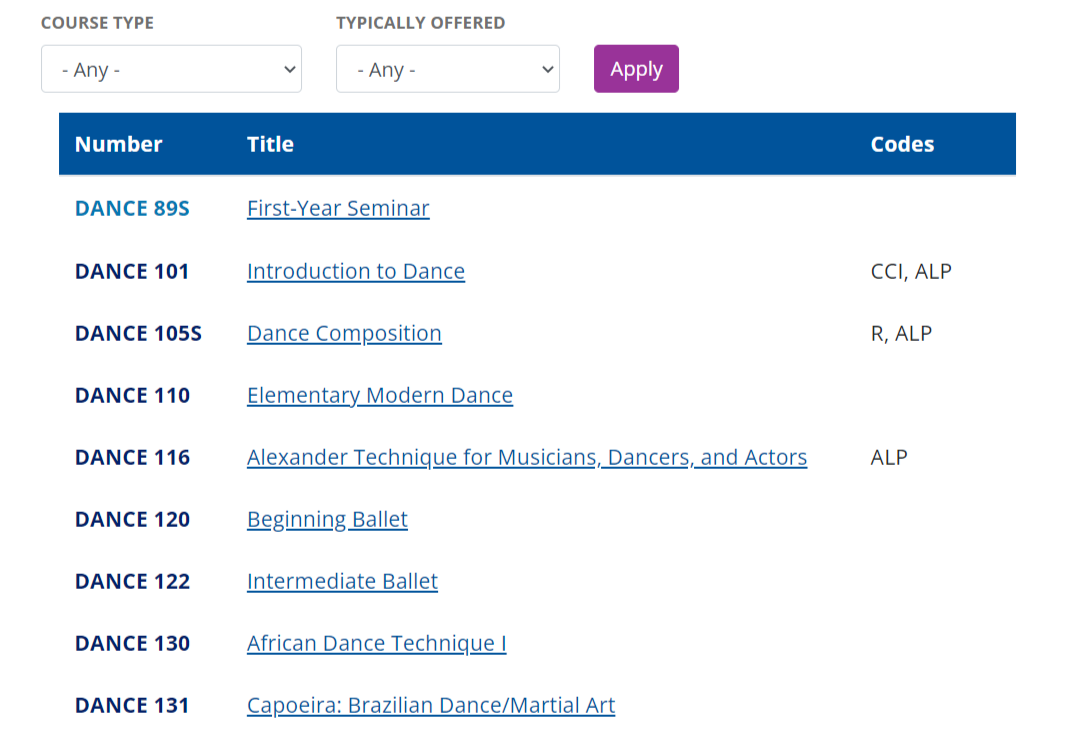
\includegraphics[scale=0.3]{slike/opis_1.png}
	\caption{Primjer prikaza tečajeva}
	\label{fig:screenshot001}
\end{figure}

Nakon što odabere željeni tečaj, klijentu se prikazuju informacije o odabranom tečaju, primjerice, vrsta plesa, kalendar te ime, prezime i slika trenera. Ponovno sličnu mogućnost nalazimo na \url{https://danceprogram.duke.edu/courses/dance-composition}, gdje, kad odaberemo tečaj, prikažu nam se neke informacije o tečaju, u ovom slučaju, vrsta plesa i razdoblje godine u kojem se taj tečaj izvodi, međutim, na ranije spomenutoj web stranici, pri odabiru tečaja, ne nalazimo informacije o treneru i kalendar, što je jedna od odlika projektne aplikacije.

\begin{figure}[H]
	\centering
	
\includegraphics[scale=0.3]{slike/opis_2.png}
	\caption{Primjer prikaza informacija o tečajevu}
	\label{fig:screenshot002}
\end{figure}

U kalendaru korisnik može pregledati sve zapisane termine tečaja i njihovu lokaciju s dvoranom. Također, klijent može pregledati i aktivne prijave za tečaj od određenog kluba i prijaviti se na njih.

\underbar{Klubovi} organiziraju plesnjake koji se mogu izvoditi i na lokacijama van kluba, a sadrže naziv, opis i sliku. Plesnjaci nisu ograničeni na samo jedan tip plesa, već je moguće plesati više različitih vrsta plesova.

Na profilu kluba se nalaze informacije o imenu kluba, broj telefona, kratki opis, poveznica na stranicu s grupama za upis, popis plesova koje njihovi treneri nude, prikaz lokacija na karti te popis dvorana po lokacijama.

Plesni Klub Tina, na poveznici \url{https://www.plesniklubtina.hr/}, korisnicima također nudi informacije o imenu kluba, broj telefona, kratki opis i lokaciju, koja, za razliku od projektne aplikacije, nije prikazana na karti. Također, za razliku od projektne aplikacije, 'Tina' korisnicima prikazuje svoj mail i sponzora, dok s druge strane ne nudi poveznicu na stranicu s grupama za upis, popis plesova u svom repertoaru i popis dvorana.

\begin{figure}[H]
	\centering
	
\includegraphics[scale=0.2]{slike/opis_3.png}
	\caption{Primjer opisa kluba}
	\label{fig:screenshot003}
\end{figure}

Klub može objaviti upise za tečaj s krajnjim rokom za prijavu, te može ograničiti upis u grupu postavljanjem dobne granice ili ograničavanjem upisa na samo jedan spol. Zatim se grupi dodjeljuje trener, skup treninga kroz neko vrijeme, gornja granica broja sudionika, te mnoge informacije koje klijentu mogu pomoći pri odabiru grupe, primjerice težina treninga, posebni uvjeti treniranja i pravila ponašanja. Nakon isteka roka, klub radi selekciju prijavljenih klijenata za grupu. Klub može naknadno mijenjati popis klijenata te uređivati i brisati grupe.

Jedna od zadaća kluba je također izbor trenera.

Ulogu \underbar{trenera} može dobiti i obnašati bilo koji klijent koji određenom klubu pošalje prijavu, motivacijsko pismo i potvrdu u obliku pdf dokumenta da je sposoban držati tečaj plesa, te ga zatim isti klub i potvrdi. Svaki trener ima podstranicu na kojoj se nalazi popis svih grupa koje trenira, a termine može pronaći u kalendaru. Na stranici \url{https://danceprogram.duke.edu/courses} također nailazimo na podstranice trenera, čiji je sadržaj potpuno drugačiji od sadržaja podstranice trenera projektne aplikacije, primjerice, na projektnoj web aplikaciji ne nailazimo na detaljan opis trenera, njegovog školovanja i kompetencija, te broj za kontakt. Projektna web aplikacija također ne sadrži sliku trenera na njegovoj podstranici.

\begin{figure}[H]
	\centering
	
\includegraphics[scale=0.3]{slike/opis_4.png}
	\caption{Primjer podstranice o treneru}
	\label{fig:screenshot004}
\end{figure}

Trener, nakon otvaranja tečaja, uz opće informacije, dobije i popis klijenata koji su potvrdili svoj dolazak na tečaj.

\underbar{Administrator} ima najveće ovlasti. On ima mogućnost mijenjanja, dodavanja i brisanja plesova. Plesovi sadrže naziv, kratki opis, sliku i link na video primjer dotičnog plesa. Također, administrator može pregledati popis svih klijenata i klubova te istima uređivati korisničke račune.

Uz manje promjene, ova web aplikacija može imati širok spektar uporabe. Uz ovakvu implementaciju, neće ju biti teško izmjeniti da pokrije neka druga područja. Primjerice, ukoliko stavimo nogometni klub, trening, nogometni tečaj i vrstu treninga u ulogu plesnog kluba, plesnjaka, plesnog tečaja i plesa, uz neznatne adaptacije ova aplikacija će biti transformirana u web aplikaciju koja nogometašima olakšava pronalazak nogometnog kluba. Osim u svijetu sporta, ova web aplikacija može se adaptirati da postane pogodna za razne umjetnosti. Zamjenimo li plesni klub sa školom slikanja, plesnjak sa satom slikanja, tečaj plesa s tečajem slikanja a ples sa tehnikom slikanja, dobit ćemo web aplikaciju koja uživateljima slikanja olakšava pronalaženje pogodnih tečajeva i škola. Također, ova web aplikacija može prilagodbom postati aplikacija za pronalaženje škola i tečajeva za strane jezike, aplikacija za pronalaženje raznih volonterskih udruga i slično.

Zbog svoje jednostavnosti, ovu web aplikaciju je vrlo lako nadograditi da korisniku nudi brojne druge funkcionalnosti. Primjerice, uz određene adaptacije na klijentskoj i poslužiteljskoj strani, klijentu se može omogućiti davanje ocjene klubu, koja se uračuna u dosadašnje ocjene tog kluba i prikazuje korisnicima na stranici kluba, čime bi korisnici mogli jasno vidjeti koliko su prijašnji polaznici tečajeva tog kluba bili zadovoljni s njim. Također, web aplikacija bi se mogla nadograditi tako da sadrži forum u kojem korisnici raspravljaju o plesovima i tečajevima, čime bi se korisnicima omogućilo sklapanje novih prijateljstava i diskutiranje o svom hobiju.		
	
